% !TEX root = main.tex

% TODO:
% REMARK:

\section{Physical Objects Reconstruction and Selection}
\label{sec:PhysObj}

	\subsection{Vertex}
	\label{ssec:PhysObj_vertex}

		% https://iopscience.iop.org/article/10.1088/1742-6596/110/9/092009/pdf

	\subsection{Pileup Issue}
	\label{ssec:PhysObj_pu}{}

		% https://cms.cern/news/reconstructing-multitude-particle-tracks-within-cms
		Because of the high luminosity of pp collision in CMS, there are more than one pp collision occuring in every time when the the bunches cross one another. The multiple collision in one crossing event is called $\textbf{pile-up(pileup)}$. In the present, the LHC is operating at an instantaneous luminosity of $0.7\times10^{34} cm^{-2}s^{-1}$, and the proton bunches cross inside CMS every 50 ns, so there are more proton in one bunch and showing high pileup. Also, the high granularity and efficiency of CMS Tracker make them distinguish the many tracks in an event. The pileup image is shown below(Fig.\ref{PhysObj:fig:pileup_img}).

		% https://cms.cern/news/reconstructing-multitude-particle-tracks-within-cms
		\begin{figure}[H]
		\centering{}
	    	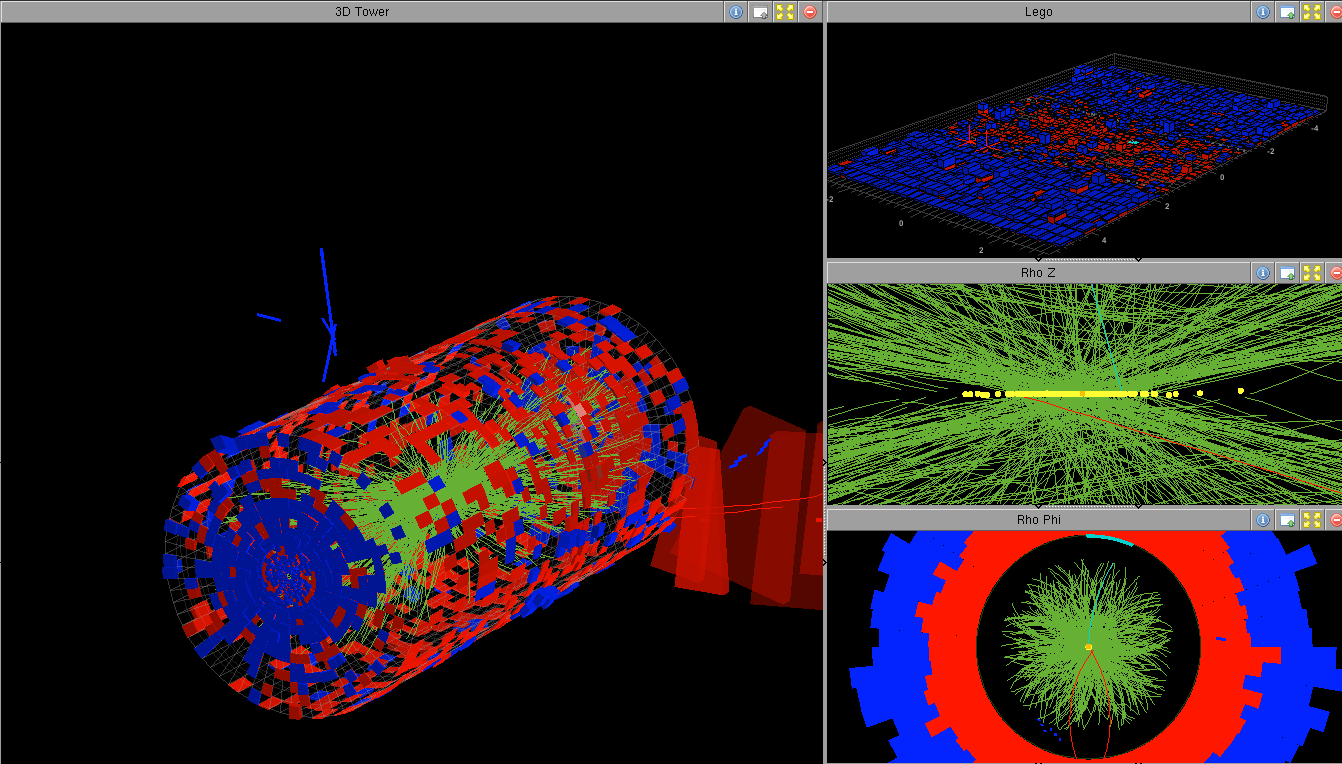
\includegraphics[width=0.85\textwidth]{Figures/PhysObj/pileup_image.png}\\
		\caption{78 reconstructed vertices in one crossing from high pileup run (3D, lego, on Pho-z plane, on Rho-Phi plane)}
		\label{PhysObj:fig:pileup_img}
		\end{figure}
		\FloatBarrier



	\subsection{Lepton}
	\label{ssec:PhysObj_lep}

		The selected lepton in the analysis is required to obey the criteria of one passed $\emph{selected lepton}$ and zero $\emph{veto lepton}$ passed. The veto criteria means that there would be no lepton passing the veto criteria except the selected one. In other words, the veto criteria can filter the physical objects which are lepton-like but not really like after reconstructed from particle level to detector level. The selected criteria corresponds to tight lepton's criteria, and veto criteria follows loose lepton's criteria:

		\subsubsection{Muon}
		\label{sssec:Muon}
			

		\subsubsection{Electron}
		\label{sssec:Electron}

	\subsection{Jet}
	\label{ssec:PhysObj_jet}

		% Jet reco : Atkin_2015_J._Phys.__Conf._Ser._645_012008
		% anti-k algo : M. Cacciari, G. P. Salam, and G. Soyez, “The anti-k(t) jet clustering algorithm”, JHEP 04, 063 (2008)

		Jet is a type of physical object in high energy collider/detector physics. There are cluster of stable particles after collision, then fragmentating and hadronizing to be a jet. In the process, the strong interaction quarks and gluons cause the showering of these particles. And there is also some algorithm to reconstruct the showering to be an object -- jet, by some calormeter's and tracker's information.
		The used algorithm is anti-k algorithm to reconstruct all jets. The algorithm summarization is shown follow. First, there is a list of particles which are candidates of jets' member, they are called protojet. Secondly, for any i-th protojet, we find the minimum $d_{ij}$ and minimum $d_{iB}$ in the list. The $d_{ij}$ and $d_{iB}$ are defined below:

		\begin{equation}
		\begin{split}
		d_{ij} = min(P_{Ti}^{2p}, P_{Tj}^{2p}) \frac{\Delta_{ij}}{R^2}\\
		, \Delta_{ij} = \sqrt{ (\eta_i - \eta_j)^2 + (\phi_i - \phi_j)^2 }\\
		d_{iB} = P_{Ti}^{2p}
		\end{split}
		\label{eq:jet_reco_algo}
		\end{equation}
		\FloatBarrier

		In the definition, $P_{T}$, $\eta$ and $\phi$ individually means the transverse momentum, rapidity and azimuth of protojet. Also, the $\Delta_{ij}$ means the distance between i-th protojet and j-th protojet under $\eta$-$\phi$ space. Besides the radius parameter R, the p is the important parameter which decide the power of energy scale. The following step is to compare the minimum $d_{ij}$ and minimum $d_{iB}$, if the min-$d_{ij}$ is smaller than min-$d_{iB}$, then remove i-th and j-th protjets out of the list, and combine the i-th and j-th protojets into a new protojet and add in the original protojet list; if the min-$d_{ij}$ is larger than min-$d_{iB}$, then the i-th protojet is considered as a jet and remove it from the list of portojets. And then, choose the new i-th protojet and do the previous comparison and assignment again and again. The algorithm stops as long as the list of protojets is empty. The illustration example of algorithm is shown below(Fig.\ref{PhysObj:fig:jet_algo}). Furthermore, in CMS we commonly apply R by 0.4 as the AK4 jet, which is also used in the analysis. If the parameter p=1, it is called inclusive $k_{t}$ algorithm; and if p=0, Cambridge/Aachen algorithm; and if p=-1, anti-$k_{t}$ jet-clustering algorithm. For CMS, it used to use p=-1 case -- anti-$k_{t}$ algorithm to construct jets.

		\begin{figure}[H]
		\centering{}
	    	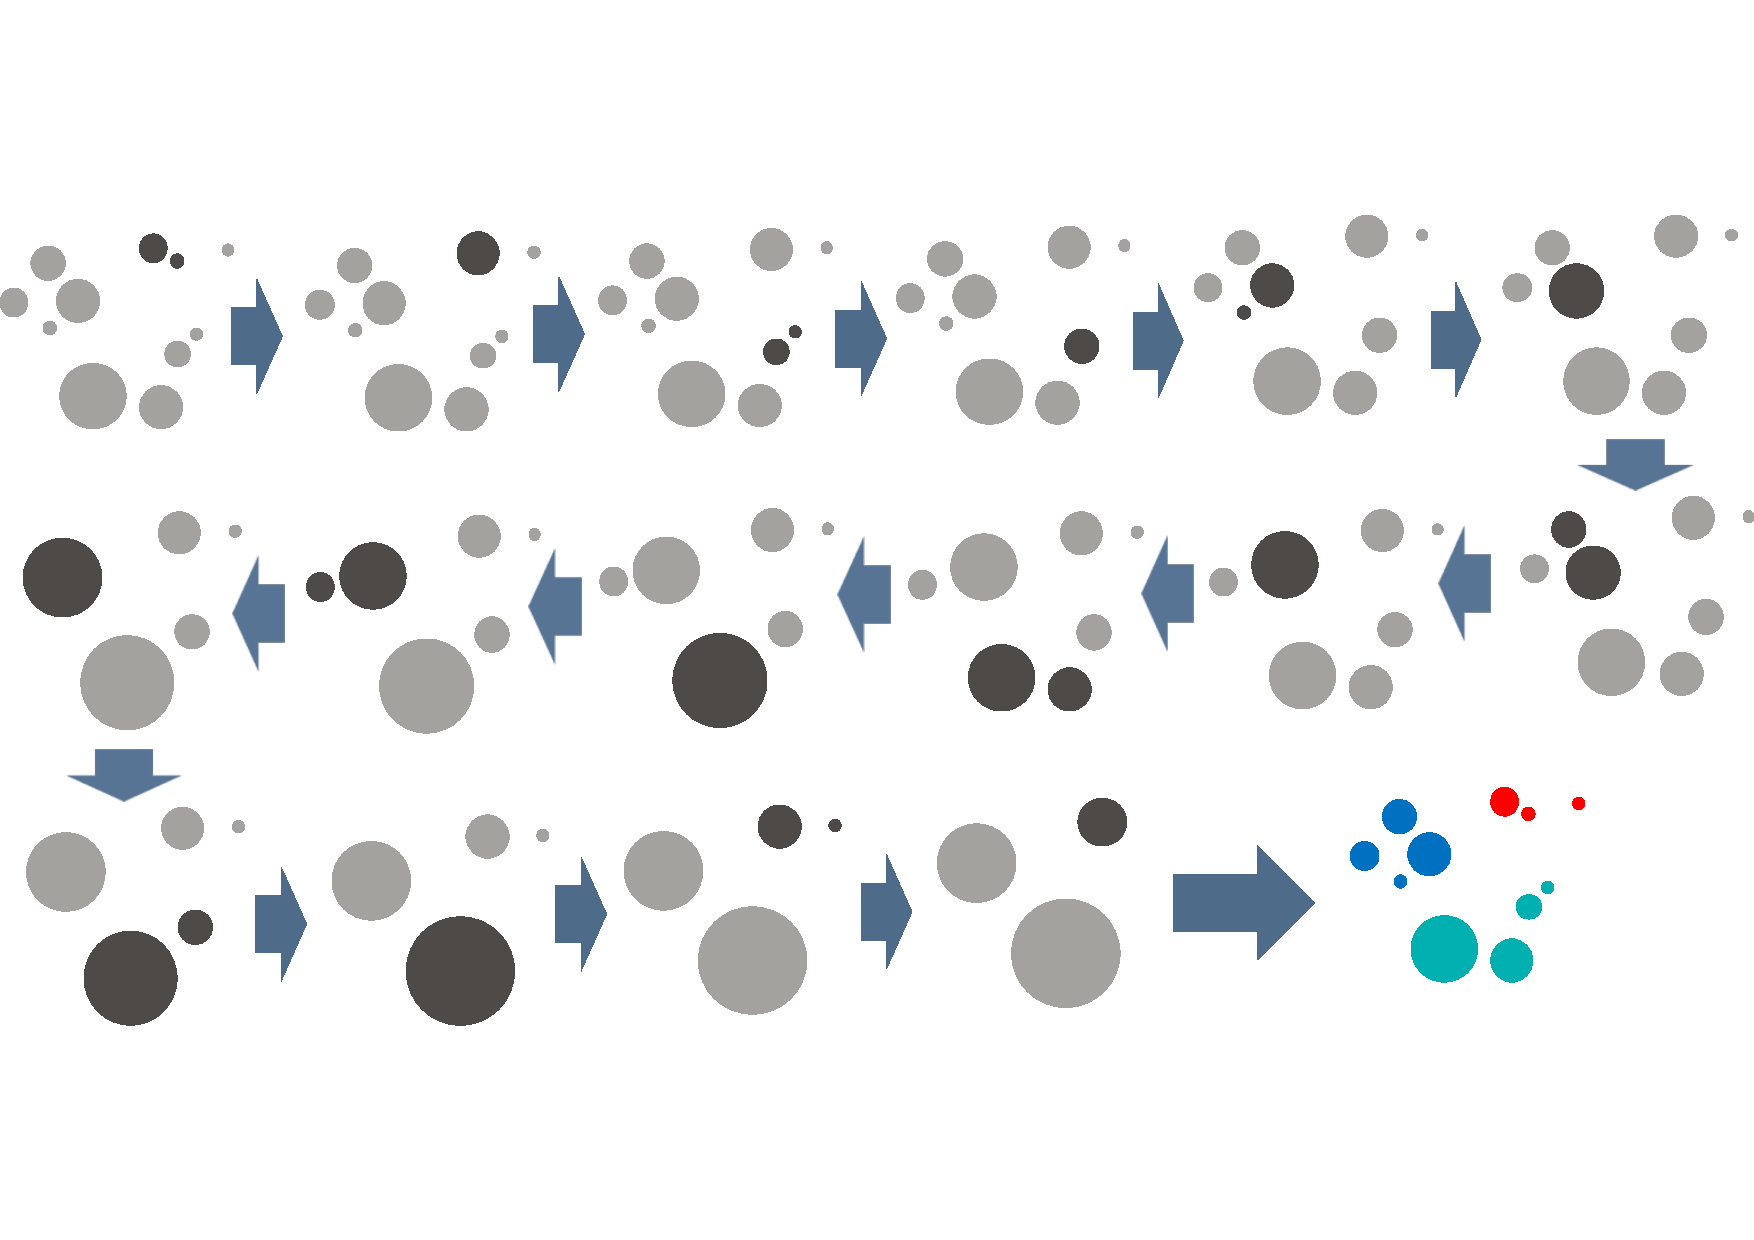
\includegraphics[width=0.85\textwidth]{Figures/PhysObj/jet_algo.pdf}\\
		\caption{Example of constructing protojets to jets}
		\label{PhysObj:fig:jet_algo}
		\end{figure}
		\FloatBarrier

		The p 


		\subsubsection{B-tagged jet}
		\label{sssec:bjet}


	\subsection{Trigger}
	\label{ssec:PhysObj_trg}





\FloatBarrier
